% Options for packages loaded elsewhere
% Options for packages loaded elsewhere
\PassOptionsToPackage{unicode}{hyperref}
\PassOptionsToPackage{hyphens}{url}
\PassOptionsToPackage{dvipsnames,svgnames,x11names}{xcolor}
%
\documentclass[
  british,
  a4paper,
]{article}
\usepackage{xcolor}
\usepackage{amsmath,amssymb}
\setcounter{secnumdepth}{-\maxdimen} % remove section numbering
\usepackage{iftex}
\ifPDFTeX
  \usepackage[T1]{fontenc}
  \usepackage[utf8]{inputenc}
  \usepackage{textcomp} % provide euro and other symbols
\else % if luatex or xetex
  \usepackage{unicode-math} % this also loads fontspec
  \defaultfontfeatures{Scale=MatchLowercase}
  \defaultfontfeatures[\rmfamily]{Ligatures=TeX,Scale=1}
\fi
\usepackage{lmodern}
\ifPDFTeX\else
  % xetex/luatex font selection
\fi
% Use upquote if available, for straight quotes in verbatim environments
\IfFileExists{upquote.sty}{\usepackage{upquote}}{}
\IfFileExists{microtype.sty}{% use microtype if available
  \usepackage[]{microtype}
  \UseMicrotypeSet[protrusion]{basicmath} % disable protrusion for tt fonts
}{}
\makeatletter
\@ifundefined{KOMAClassName}{% if non-KOMA class
  \IfFileExists{parskip.sty}{%
    \usepackage{parskip}
  }{% else
    \setlength{\parindent}{0pt}
    \setlength{\parskip}{6pt plus 2pt minus 1pt}}
}{% if KOMA class
  \KOMAoptions{parskip=half}}
\makeatother
% Make \paragraph and \subparagraph free-standing
\makeatletter
\ifx\paragraph\undefined\else
  \let\oldparagraph\paragraph
  \renewcommand{\paragraph}{
    \@ifstar
      \xxxParagraphStar
      \xxxParagraphNoStar
  }
  \newcommand{\xxxParagraphStar}[1]{\oldparagraph*{#1}\mbox{}}
  \newcommand{\xxxParagraphNoStar}[1]{\oldparagraph{#1}\mbox{}}
\fi
\ifx\subparagraph\undefined\else
  \let\oldsubparagraph\subparagraph
  \renewcommand{\subparagraph}{
    \@ifstar
      \xxxSubParagraphStar
      \xxxSubParagraphNoStar
  }
  \newcommand{\xxxSubParagraphStar}[1]{\oldsubparagraph*{#1}\mbox{}}
  \newcommand{\xxxSubParagraphNoStar}[1]{\oldsubparagraph{#1}\mbox{}}
\fi
\makeatother


\usepackage{longtable,booktabs,array}
\newcounter{none} % for unnumbered tables
\usepackage{calc} % for calculating minipage widths
% Correct order of tables after \paragraph or \subparagraph
\usepackage{etoolbox}
\makeatletter
\patchcmd\longtable{\par}{\if@noskipsec\mbox{}\fi\par}{}{}
\makeatother
% Allow footnotes in longtable head/foot
\IfFileExists{footnotehyper.sty}{\usepackage{footnotehyper}}{\usepackage{footnote}}
\makesavenoteenv{longtable}
\usepackage{graphicx}
\makeatletter
\newsavebox\pandoc@box
\newcommand*\pandocbounded[1]{% scales image to fit in text height/width
  \sbox\pandoc@box{#1}%
  \Gscale@div\@tempa{\textheight}{\dimexpr\ht\pandoc@box+\dp\pandoc@box\relax}%
  \Gscale@div\@tempb{\linewidth}{\wd\pandoc@box}%
  \ifdim\@tempb\p@<\@tempa\p@\let\@tempa\@tempb\fi% select the smaller of both
  \ifdim\@tempa\p@<\p@\scalebox{\@tempa}{\usebox\pandoc@box}%
  \else\usebox{\pandoc@box}%
  \fi%
}
% Set default figure placement to htbp
\def\fps@figure{htbp}
\makeatother



\ifLuaTeX
\usepackage[bidi=basic,shorthands=off]{babel}
\else
\usepackage[bidi=default,shorthands=off]{babel}
\fi
\ifLuaTeX
  \usepackage{selnolig} % disable illegal ligatures
\fi


\setlength{\emergencystretch}{3em} % prevent overfull lines

\providecommand{\tightlist}{%
  \setlength{\itemsep}{0pt}\setlength{\parskip}{0pt}}



 


\makeatletter
\@ifpackageloaded{tcolorbox}{}{\usepackage[skins,breakable]{tcolorbox}}
\@ifpackageloaded{fontawesome5}{}{\usepackage{fontawesome5}}
\definecolor{quarto-callout-color}{HTML}{909090}
\definecolor{quarto-callout-note-color}{HTML}{0758E5}
\definecolor{quarto-callout-important-color}{HTML}{CC1914}
\definecolor{quarto-callout-warning-color}{HTML}{EB9113}
\definecolor{quarto-callout-tip-color}{HTML}{00A047}
\definecolor{quarto-callout-caution-color}{HTML}{FC5300}
\definecolor{quarto-callout-color-frame}{HTML}{acacac}
\definecolor{quarto-callout-note-color-frame}{HTML}{4582ec}
\definecolor{quarto-callout-important-color-frame}{HTML}{d9534f}
\definecolor{quarto-callout-warning-color-frame}{HTML}{f0ad4e}
\definecolor{quarto-callout-tip-color-frame}{HTML}{02b875}
\definecolor{quarto-callout-caution-color-frame}{HTML}{fd7e14}
\makeatother
\makeatletter
\@ifpackageloaded{caption}{}{\usepackage{caption}}
\AtBeginDocument{%
\ifdefined\contentsname
  \renewcommand*\contentsname{Table of contents}
\else
  \newcommand\contentsname{Table of contents}
\fi
\ifdefined\listfigurename
  \renewcommand*\listfigurename{List of Figures}
\else
  \newcommand\listfigurename{List of Figures}
\fi
\ifdefined\listtablename
  \renewcommand*\listtablename{List of Tables}
\else
  \newcommand\listtablename{List of Tables}
\fi
\ifdefined\figurename
  \renewcommand*\figurename{Figure}
\else
  \newcommand\figurename{Figure}
\fi
\ifdefined\tablename
  \renewcommand*\tablename{Table}
\else
  \newcommand\tablename{Table}
\fi
}
\@ifpackageloaded{float}{}{\usepackage{float}}
\floatstyle{ruled}
\@ifundefined{c@chapter}{\newfloat{codelisting}{h}{lop}}{\newfloat{codelisting}{h}{lop}[chapter]}
\floatname{codelisting}{Listing}
\newcommand*\listoflistings{\listof{codelisting}{List of Listings}}
\makeatother
\makeatletter
\makeatother
\makeatletter
\@ifpackageloaded{caption}{}{\usepackage{caption}}
\@ifpackageloaded{subcaption}{}{\usepackage{subcaption}}
\makeatother
\usepackage{bookmark}
\IfFileExists{xurl.sty}{\usepackage{xurl}}{} % add URL line breaks if available
\urlstyle{same}
% fallback for those not using the hyperref driver hyperxmp:
\makeatletter
\@ifundefined{xmpquote}{\newcommand{\xmpquote}[1]{#1}}{}
\makeatother
\hypersetup{
  pdftitle={Forecasting US core inflation from the bottom up},
  pdfauthor={Carlos Galindo},
  pdflang={en-GB},
  colorlinks=true,
  linkcolor={blue},
  filecolor={Maroon},
  citecolor={Blue},
  urlcolor={Blue},
  pdfcreator={LaTeX via pandoc}}


\title{Forecasting US core inflation from the bottom up}
\usepackage{etoolbox}
\makeatletter
\providecommand{\subtitle}[1]{% add subtitle to \maketitle
  \apptocmd{\@title}{\par {\large #1 \par}}{}{}
}
\makeatother
\subtitle{A component-by-component forecast, with producer prices
translated into core PCE, tested against four major banks and the
consensus}
\author{Carlos Galindo}
\date{}
\begin{document}
\maketitle


\begin{tcolorbox}[enhanced jigsaw, arc=.35mm, bottomrule=.15mm, breakable, colback=white, colframe=quarto-callout-note-color-frame, left=2mm, leftrule=.75mm, opacityback=0, rightrule=.15mm, toprule=.15mm]

\vspace{-3mm}\textbf{At a glance}\vspace{3mm}

\begin{itemize}
\tightlist
\item
  \textbf{Question.} Can a forecast built up from individual price
  components, and from producer prices passed through to consumer
  prices, track US core inflation as well as the professional
  forecasters who publish ahead of each release?
\item
  \textbf{Approach.} Rebuilt and improved the component-level forecasts
  and the producer-price-to-core-PCE translation, then scored them out
  of sample against four major banks and the survey consensus.
\item
  \textbf{Finding.} Over October 2023 to September 2024, accuracy sat
  within the banks' range and slightly behind the consensus median.
\item
  \textbf{Why it matters.} A transparent bottom-up forecast explains
  \emph{where} an inflation surprise comes from, which a single
  aggregate number cannot.
\end{itemize}

\end{tcolorbox}

\subsection{The question}\label{the-question}

Core inflation, which strips out food and energy, is what central banks
watch most closely, and the United States publishes it in two main
forms: the consumer price index, released first, and the personal
consumption expenditures price index, released a few weeks later and the
one the Federal Reserve targets. Forecasters publish their expectations
for each month's print in advance. A survey of those forecasts gives a
consensus, and the consensus is hard to beat: it pools many informed
judgements, most of them made with the latest data and a sense of how
each category has behaved lately.

A forecast of the aggregate can be built in two ways. The first models
the aggregate directly. It is simple, but when it misses it says little
about why. The second builds up from the pieces: dozens of price
categories such as used cars, airfares, rents, medical services and
apparel, each with its own dynamics and its own drivers, combined with
the weights that statisticians use to construct the headline. When the
headline surprises, a bottom-up forecast can say which categories moved
and whether the movement looks like noise, a one-off, or a trend.

There is a second link that matters for the personal consumption
measure. Many of its components are not priced from consumer surveys at
all. They are derived from producer prices, such as margins earned by
retailers and wholesalers, or prices charged by medical providers.
Because producer prices are released a few days before the consumption
series is published, they allow a forecaster to sharpen a core PCE
nowcast just before the print. The question here is whether a rebuilt
version of both pieces, the component forecasts and the producer-price
translation, performs credibly against the people who do this for a
living.

\subsection{Approach}\label{approach}

The work was begun in a previous role and rebuilt and improved during
the career break. The rebuild kept the architecture and changed what sat
inside it.

\textbf{Component forecasts.} Each price category has its own monthly
equation, estimated on month-on-month changes. A candidate set of
regressors enters every equation: up to thirteen of the category's own
monthly lags, calendar effects for month and quarter, and a large panel
of external indicators. These cover other consumer price categories,
producer price indices at several levels of aggregation, import prices,
financial-market variables such as yields and equity prices, housing
indicators, and survey-based price measures. Selection is stepwise, in
two stages. A first, looser pass screens the candidates. A second,
stricter pass then chooses from what survived. The final equation is
re-estimated with a structural-break check so that one unusual stretch
of history does not drive the coefficients, and where an estimate fails
the model falls back to a robust estimator. The point of two stages is
to keep a wide search while resisting the spurious fits that a single
wide search produces.

\textbf{From producer prices to core PCE.} The translation works at the
level of the personal consumption measure itself. Candidate predictors,
including the producer-price aggregates and the category-level forecasts
from the first block, are added one at a time. An addition is kept only
while its coefficient remains significant at the ten per cent level, up
to a fixed ceiling of additions. Each step yields a forecast, and the
set of forecasts is then pooled, using weights estimated from how well
each has performed. The pooled path is seasonally adjusted with a
model-based adjustment procedure so that it is comparable with the
published series. Pooling was chosen deliberately. It is the same lesson
the wider forecasting literature reports: individual models are
unstable, and an average of reasonable models is more reliable than any
chosen one.

\textbf{Testing.} The forecasts were scored out of sample: each month's
forecast used only information available at the time, and was compared
with the realised print. The comparison group was four major banks that
publish individual monthly forecasts, plus the survey's median, over the
twelve months from October 2023 to September 2024. The consensus data is
Bloomberg survey data (2024). It is licensed, so this note reports only
summary findings.

\subsection{What the work shows}\label{what-the-work-shows}

The headline finding is modest, and stated plainly: across October 2023
to September 2024, the bottom-up forecasts landed within the range of
the four banks, and slightly behind the consensus median. Being inside
the banks' range means the rebuilt system was not an outlier; on some
months it was closer to the outcome than some banks, on others further.
Being slightly behind the consensus median is the usual result for any
single forecaster, because the median benefits from averaging out
individual errors. The evidence does not support a claim that the system
beats professional forecasters. It supports the narrower claim that a
transparent, rebuilt system built by one researcher is competitive with
them.

The simulated figure below shows what such a scoring exercise looks
like. The real comparison used the same structure: twelve monthly
prints, four bank forecasts and a consensus median, and one model. The
paths here are generated, so they show how the output is read, not what
the real forecasts were.

\begin{figure}

\centering{

\pandocbounded{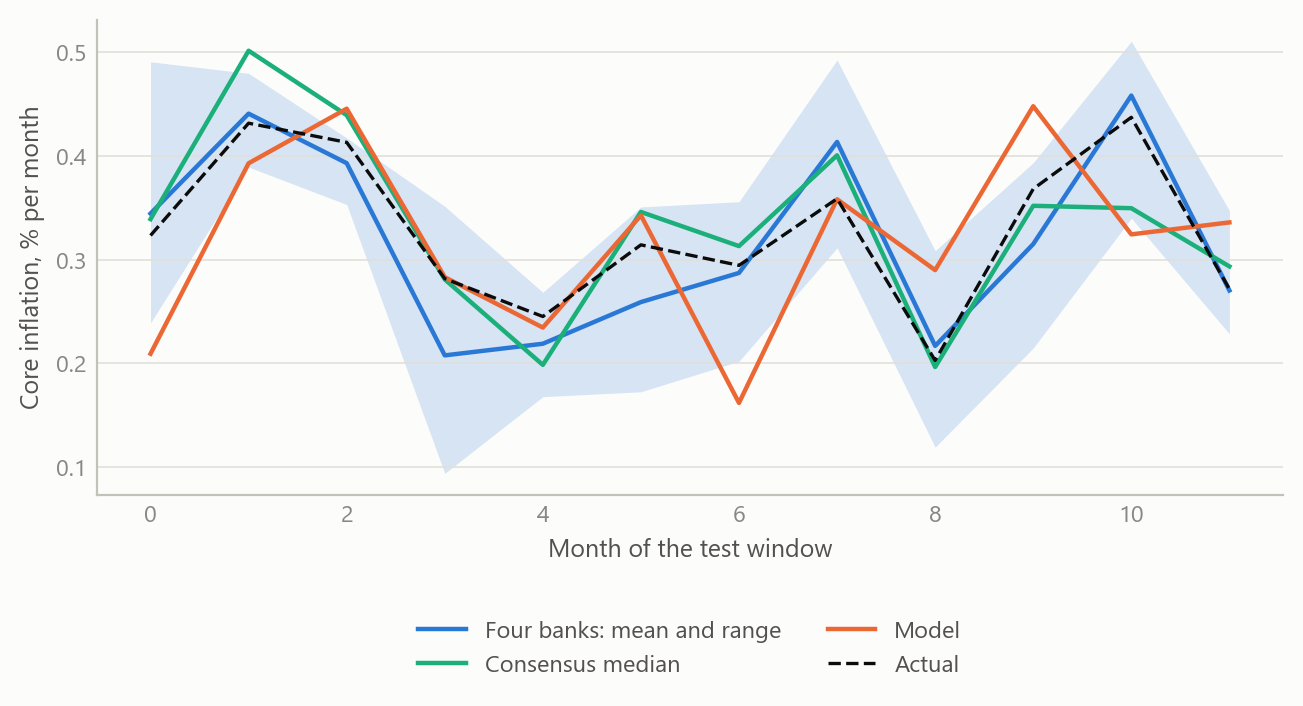
\includegraphics[keepaspectratio]{index_files/figure-latex/fig-scoring-output-1.png}}

}

\caption{\label{fig-scoring}Out-of-sample scoring layout: actual monthly
core inflation, the range of four bank forecasts, the consensus median
and a model forecast over twelve months (simulated data).}

\end{figure}%

The second figure shows the logic of building up from components. In any
one month, each category contributes its weight times its forecast
change, and the headline forecast is the sum. The useful property is
that the contributions can be inspected one by one.

\begin{figure}

\centering{

\pandocbounded{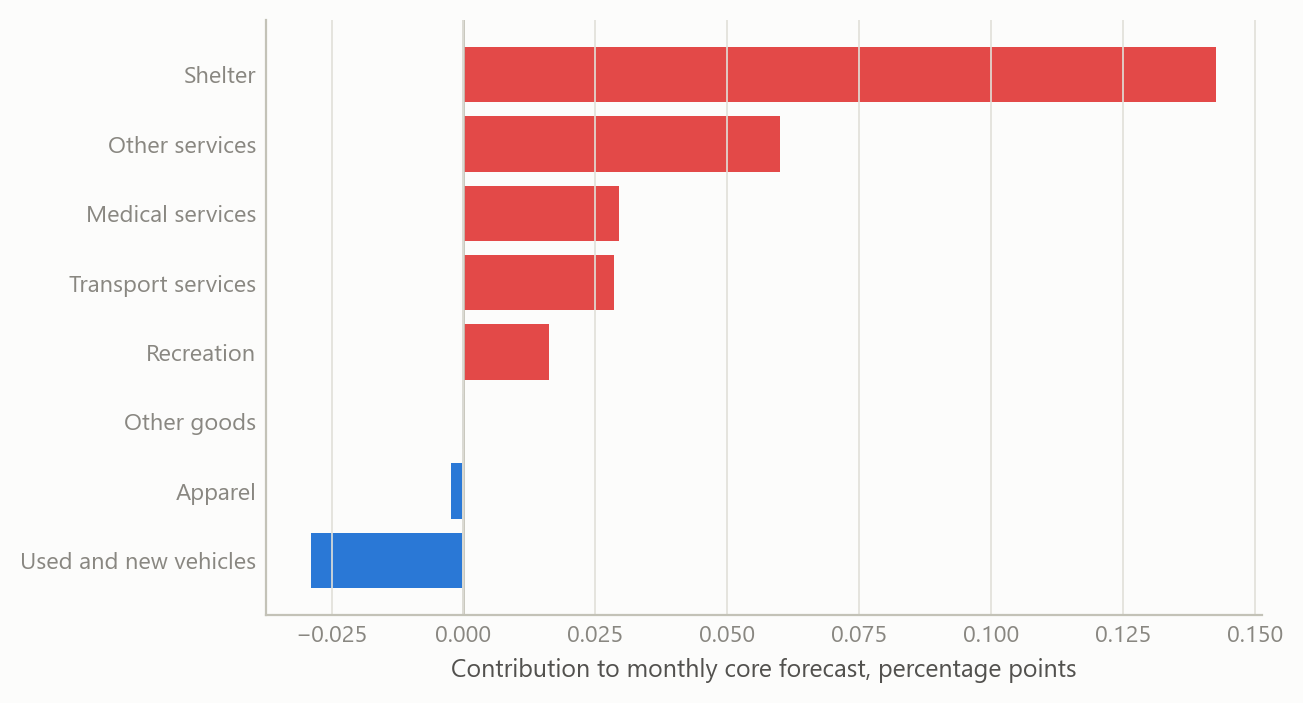
\includegraphics[keepaspectratio]{index_files/figure-latex/fig-components-output-1.png}}

}

\caption{\label{fig-components}Contribution of broad price groups to a
core forecast in one month: weight times forecast monthly change
(simulated data).}

\end{figure}%

The third figure shows the producer-price link. Producer-price changes
feed consumer prices with a delay, and the strength of the link differs
across the delay. The forecast uses the profile of that delay to decide
how much weight a fresh producer-price release deserves.

\begin{figure}

\centering{

\pandocbounded{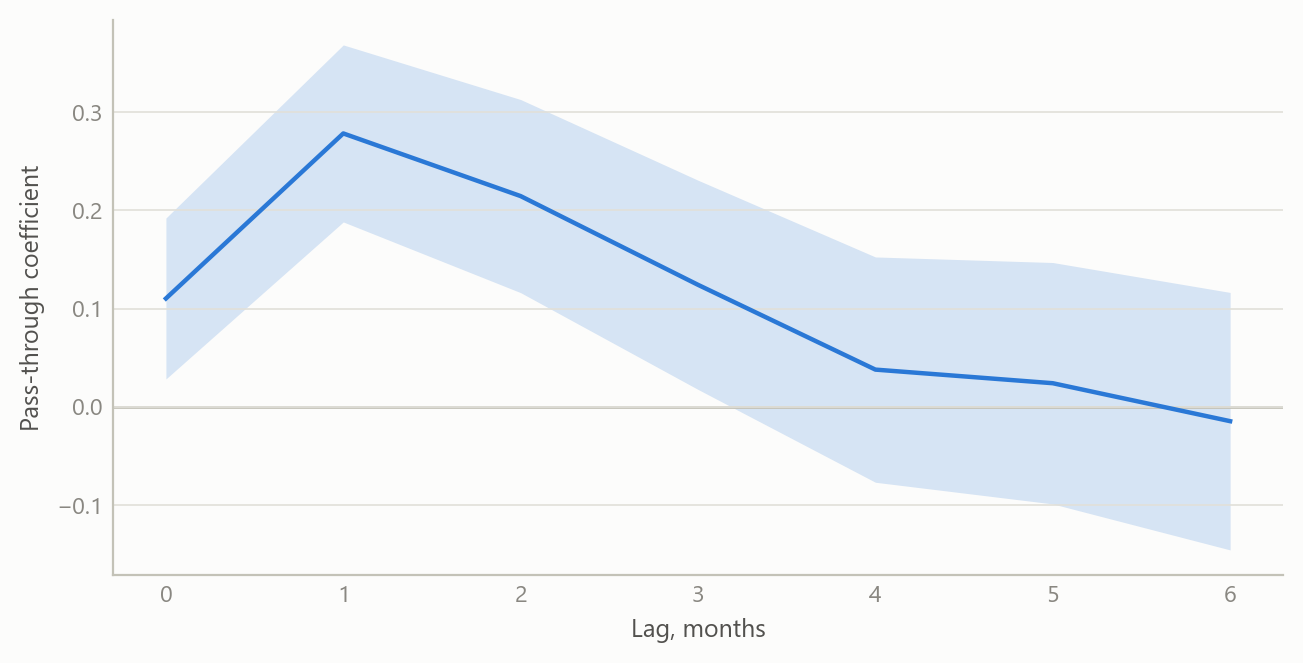
\includegraphics[keepaspectratio]{index_files/figure-latex/fig-lag-output-1.png}}

}

\caption{\label{fig-lag}Illustrative lag profile: association between a
producer-price margin series and a core PCE category at lags of zero to
six months, with simulated uncertainty bands (simulated data).}

\end{figure}%

\subsection{Insights}\label{insights}

\textbf{A forecast that can be taken apart is worth more than a forecast
that is slightly more accurate.} Staying within the banks' range, with a
clear account of each category's contribution, is more useful to a user
than a black-box number of the same accuracy. When the print arrives,
the bottom-up view says which components accounted for the miss.

\textbf{Wide search needs a stricter second pass.} A large indicator
panel will always produce good in-sample fits. Two-stage selection,
break checks and a robust fallback reduce the share of those fits that
are accidents of the sample.

\textbf{Pooling earns its place.} The consensus median is a pooled
forecast, and it was ahead of the single system. The system itself pools
many specifications for the same reason. Where weighting by past
accuracy is available, it is a cheap and effective step.

\textbf{Producer prices are timely, and timing is the point.} The
producer-price release precedes the consumption price release, so the
translation is most useful in the days before the print, when the other
forecasters are also updating. That is where a small edge, if there is
one, is found.

\textbf{Transparent scoring is the discipline.} The test was against
named outside benchmarks over a defined twelve-month window, with the
result reported as it came out: competitive, and not ahead.

\subsection{Scope and next steps}\label{scope-and-next-steps}

The window is twelve monthly observations. That is enough to say the
system is not an outlier among bank forecasters, and too short to rank
it precisely against them or against the median. A difference of a few
hundredths of a percentage point per month between forecasters is within
what one or two unusual months can produce.

The test also covers a particular period, one of declining but stubborn
inflation. A bottom-up system could behave differently when relative
prices move sharply, for example in a commodity shock, and the window
does not tell us.

Two extensions would strengthen the work. First, a longer scored
history, with formal tests of equal predictive accuracy against the
consensus, so that ``slightly behind'' becomes a statement with a
confidence interval. Second, a scoring split by category, to show which
components the system forecasts best and which it should hand over to
the pooled average.

\subsection{About the evidence}\label{about-the-evidence}

The scoring window runs from October 2023 to September 2024, with the
rebuild carried out during the career break, from May 2024. The
comparison uses four bank forecasts and the survey consensus from
Bloomberg survey data (2024); the data is licensed, so only the summary
result is stated. All figures here are simulated and illustrate the
method and the scoring layout.

Figures and tables marked \emph{simulated} are generated from simulated
data built to share the structure of the analysis (its variables,
horizons and frequencies). They show how each method works and what its
output looks like. Results stated in the text, and figures that give a
source, are the project's own. Methods are described at the level of a
methods section. Code and data pipelines are not reproduced here.




\end{document}
